\documentclass{article}
\usepackage[utf8]{inputenc}
\usepackage{longtable}
\usepackage{authblk}
\usepackage{adjustbox}
\usepackage{natbib}
\usepackage{fancyhdr}
\pagestyle{fancy}
\fancyhf{}
\lhead{Nicolás Huertas -201326730}
\title{Herramientas Computacionales para la
 Investigación Interdisciplinar Reproducible  Proyecto Final}
% autores

\author[1]{\normalsize Nicolás Huertas - 201326730}


\affil[1]{\small  Departamenta de Ingeniería Industrial ,Universidad de los Andes\\
\texttt{{n.huertas10}@uniandes.edu.col}}


\date{30 de Junio de 2018}

\usepackage{Sweave}
\begin{document}
\Sconcordance{concordance:ProyectoHC.tex:ProyectoHC.Rnw:%
1 23 1 1 0 13 1 1 25 7 1 1 4 15 0 1 2 11 1 1 11 1 2 8 1 1 13 1 2 10 1 1 %
7 12 0 1 2 3 1 1 6 14 0 1 3 7 1 1 3 1 2 17 1 1 5 1 1 1 2 34 0 1 2 11 1 %
1 9 1 1 1 25 3 1 1 15 1 2 9 1}

\begin{figure}
 \centering
 
\includegraphics[width = 3cm, height=1cm]{Uandes}
\end{figure}
\maketitle
\begin{abstract}
Este proyecto busca explorar herramientas computacionales como Python, R, Zotero y LATEX para la generación de trabajo replicable. En este caso se explorarán variables de desarrollo humano para el caso Colombiano por departamento. De esta forma se identificará cuales son los departamentos que tienen mejores indices y peores asi como ver la relación entre ellos. Para esto se hara un análisis univariado que permita identificar como se comporta cada inice luego
\end{abstract}

\section*{Introducción}

Aqui les presento mi investigacion sobre diversos indices sociales en el mundo. Los indices los conseguí de wikipedia, espero que les gusten mucho. Aqui les presento mi investigacion sobre diversos indices sociales en el mundo. Los indices los conseguí de wikipedia, espero que les gusten mucho.Aqui les presento mi investigacion sobre diversos indices sociales en el mundo. Los 

 Comencemos viendo que hay en la sección \ref{univariada} en la página \pageref{univariada}.
 

\section{Exploración Univariada}\label{univariada}
 
 Para conocer el comportamiento de las variables se ha preparado la Tabla \ref{stats}, donde se describe la distribución de las modalidades de cada variable. Los números representan la situación de algun país en ese indicador, donde el mayor valor numérico es la mejor situación.
% 
% Table created by stargazer v.5.2.2 by Marek Hlavac, Harvard University. E-mail: hlavac at fas.harvard.edu
% Date and time: Fri, Jun 29, 2018 - 23:24:48
\begin{table}[!htbp] \centering 
  \caption{Medidas estadísticas} 
  \label{stats} 
\begin{tabular}{@{\extracolsep{5pt}}lccccc} 
\\[-1.8ex]\hline 
\hline \\[-1.8ex] 
Statistic & \multicolumn{1}{c}{N} & \multicolumn{1}{c}{Mean} & \multicolumn{1}{c}{Median} & \multicolumn{1}{c}{Min} & \multicolumn{1}{c}{Max} \\ 
\hline \\[-1.8ex] 
IDH & 32 & 0.802 & 0.804 & 0.691 & 0.879 \\ 
Población.Cabecera & 32 & 1,196,730.000 & 717,197 & 13,090 & 10,070,801 \\ 
Población.Resto & 32 & 360,590.300 & 268,111.5 & 21,926 & 1,428,858 \\ 
Población.Total & 32 & 1,557,320.000 & 1,028,429 & 43,446 & 10,985,285 \\ 
\hline \\[-1.8ex] 
\end{tabular} 
\end{table} % 
% 
 Como apreciamos en la Tabla \ref{stats}, los países en la mejor situación son los menos, salvo en el caso del \emph{índice de libertas mundial}\footnote{Nótese que esto se puede deber a la {\bf menor} cantidad de categorías.}
% 

% 
 Para resaltar lo anterior, tenemos la Figura \ref{barplots} en la página \pageref{barplots}. 
% 
%  
% %%%%% figure
\begin{figure}[h]
\centering
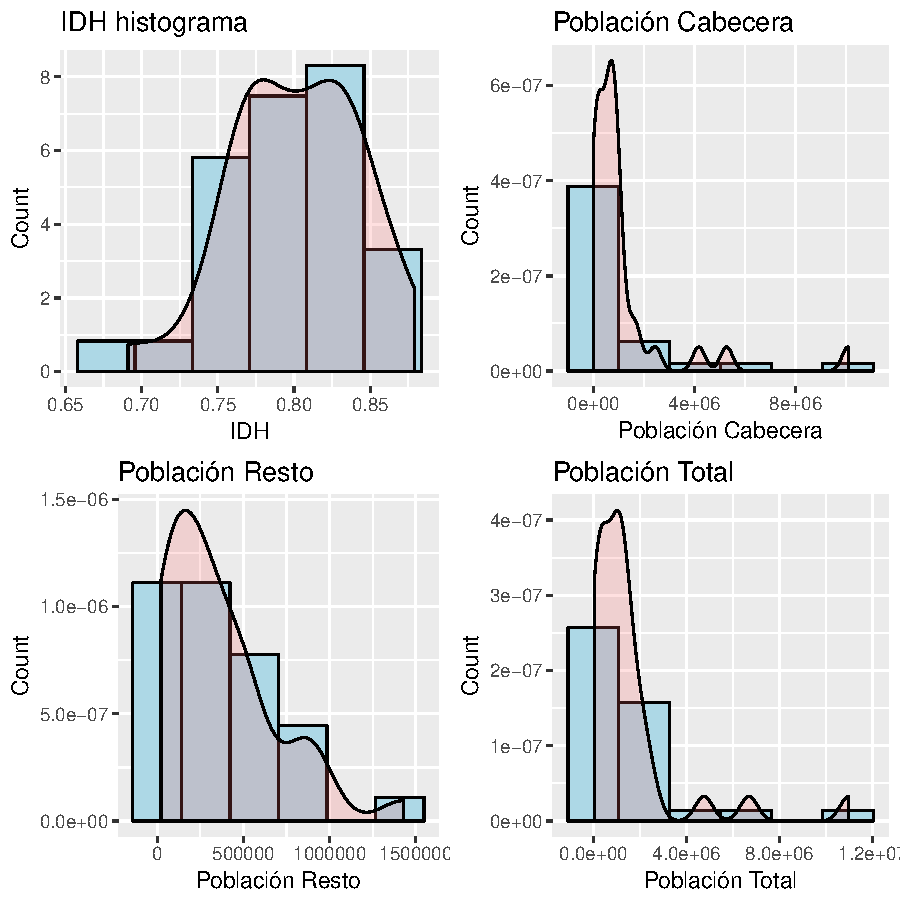
\includegraphics{ProyectoHC-barplots}
\caption{Distribución de Indicadores}
\label{barplots}
\end{figure}

dado el sesgo de las pobaciones, podriamos transformarla para que se acerque a la  normalidad
\clearpage
 \begin{figure}[h]
\centering
%\begin{adjustbox}{width=7cm,height=7cm,clip,trim=1.5cm 0.5cm 0cm 1.5cm}
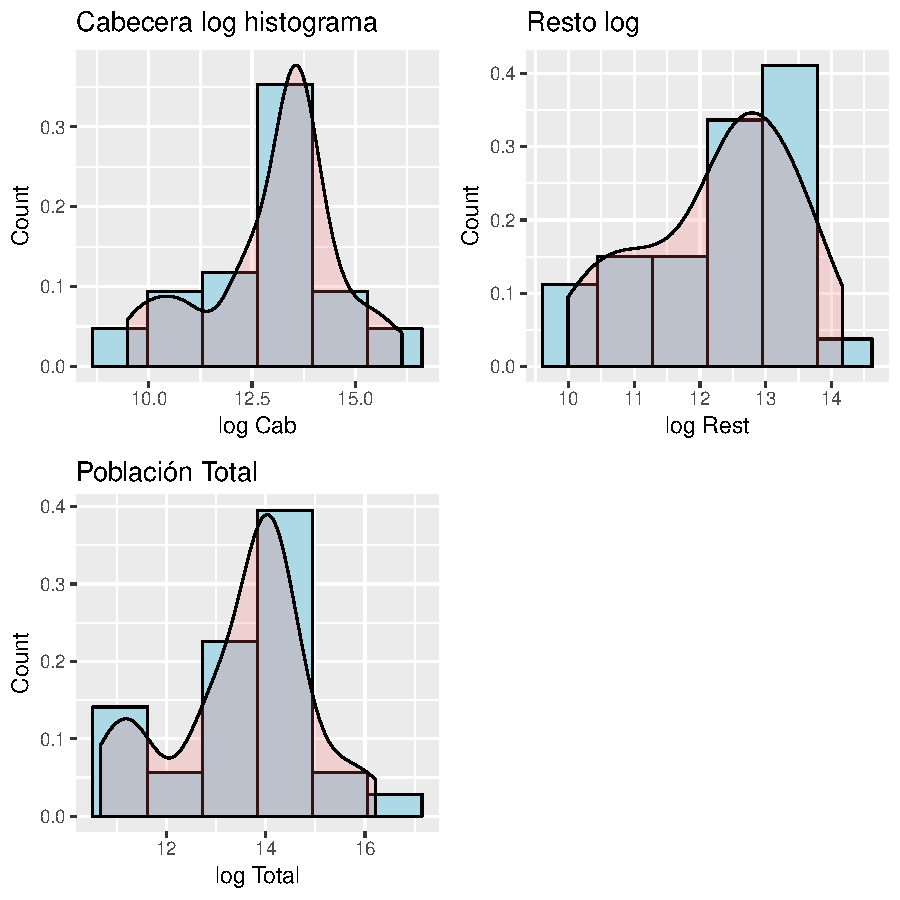
\includegraphics{ProyectoHC-barplots2}
%\end{adjustbox}
\caption{Distribución de Indicadores normalizada}
\label{barplots2}
\end{figure}
\clearpage
% 
% 
\section{Exploración Bivariada}
% 
 En este trabajo estamos interesados en el impacto de la población en el nIDH. Veamos las relaciones bivariadas que tiene esta variable con todas las demás:
% 
% Table created by stargazer v.5.2.2 by Marek Hlavac, Harvard University. E-mail: hlavac at fas.harvard.edu
% Date and time: Fri, Jun 29, 2018 - 23:24:50
\begin{table}[!htbp] \centering 
  \caption{Correlación de IDH con las demás variables} 
  \label{corrDem} 
\begin{tabular}{@{\extracolsep{5pt}} ccc} 
\\[-1.8ex]\hline 
\hline \\[-1.8ex] 
cabeLog & restoLog & totalLog \\ 
\hline \\[-1.8ex] 
$0.487$ & $0.177$ & $0.424$ \\ 
\hline \\[-1.8ex] 
\end{tabular} 
\end{table} 
% 
Veamos la correlación entre las variables independientes:
% 
% Table created by stargazer v.5.2.2 by Marek Hlavac, Harvard University. E-mail: hlavac at fas.harvard.edu
% Date and time: Fri, Jun 29, 2018 - 23:24:50
\begin{table}[!htbp] \centering 
  \caption{Correlación entre variables independientes} 
  \label{corrTableX} 
\begin{tabular}{@{\extracolsep{5pt}} cccc} 
\\[-1.8ex]\hline 
\hline \\[-1.8ex] 
 & cabeLog & restoLog & totalLog \\ 
\hline \\[-1.8ex] 
cabeLog & 1 &  &  \\ 
restoLog & 0.84 & 1 &  \\ 
totalLog & 0.99 & 0.9 & 1 \\ 
\hline \\[-1.8ex] 
\end{tabular} 
\end{table} 


Lo visto en la Tabla \ref{corrTableX} se refuerza claramente en la Figura \ref{corrPlotX}.

\begin{figure}[h]
\centering
\begin{adjustbox}{width=7cm,height=7cm,clip,trim=1.5cm 0.5cm 0cm 1.5cm}
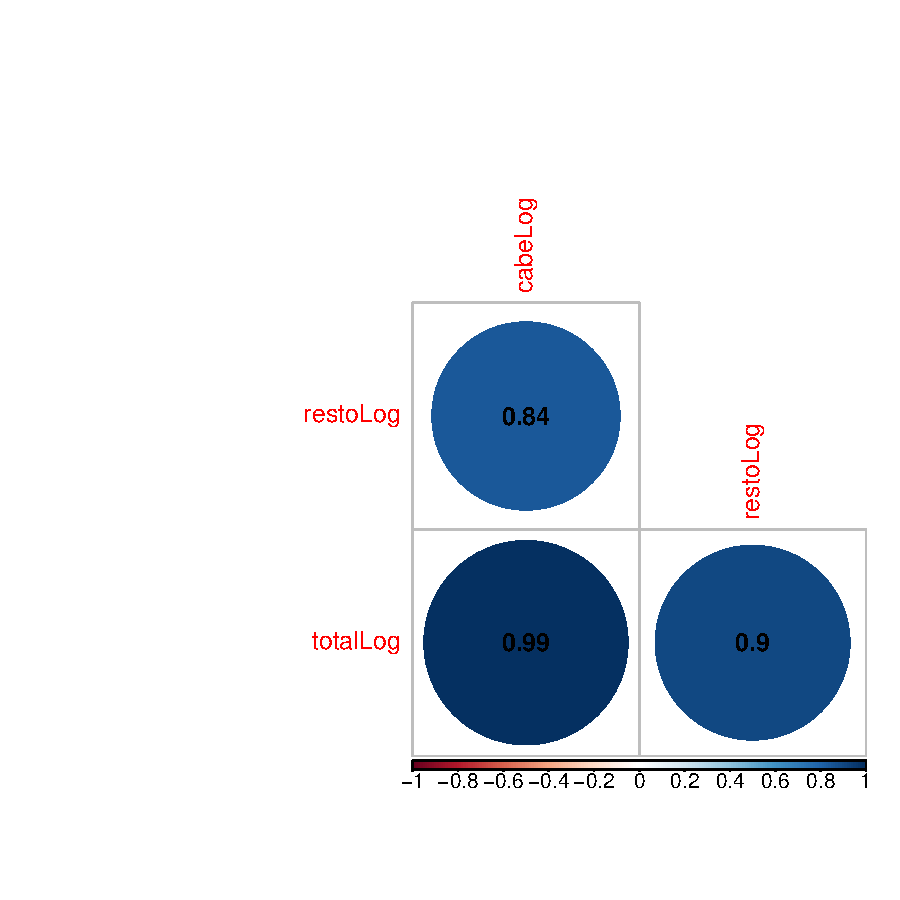
\includegraphics{ProyectoHC-corrPlotX}
\end{adjustbox}
\caption{correlación entre predictores}
\label{corrPlotX}
\end{figure}






% 
% 
\clearpage
% 
\section{Modelos de Regresión}
% 
Finalmente, vemos los modelos propuestos. Primero sin la libertad mundial como independiente, y luego con está. Los resultados se muestran en la Tabla \ref{regresiones} de la página \pageref{regresiones}.
% 
% 
% 
% Table created by stargazer v.5.2.2 by Marek Hlavac, Harvard University. E-mail: hlavac at fas.harvard.edu
% Date and time: Fri, Jun 29, 2018 - 23:24:50
\begin{table}[!htbp] \centering 
  \caption{Modelos de Regresión} 
  \label{regresiones} 
\begin{tabular}{@{\extracolsep{5pt}}lcc} 
\\[-1.8ex]\hline 
\hline \\[-1.8ex] 
 & \multicolumn{2}{c}{\textit{Dependent variable:}} \\ 
\cline{2-3} 
\\[-1.8ex] & \multicolumn{2}{c}{IDH} \\ 
\\[-1.8ex] & (1) & (2)\\ 
\hline \\[-1.8ex] 
 cabeLog & 0.013$^{***}$ & 0.066 \\ 
  & (0.004) & (0.046) \\ 
  & & \\ 
 restoLog &  & $-$0.016 \\ 
  &  & (0.020) \\ 
  & & \\ 
 totalLog &  & $-$0.051 \\ 
  &  & (0.064) \\ 
  & & \\ 
 Constant & 0.634$^{***}$ & 0.818$^{***}$ \\ 
  & (0.055) & (0.092) \\ 
  & & \\ 
\hline \\[-1.8ex] 
Observations & 32 & 32 \\ 
R$^{2}$ & 0.238 & 0.437 \\ 
Adjusted R$^{2}$ & 0.212 & 0.377 \\ 
Residual Std. Error & 0.037 (df = 30) & 0.033 (df = 28) \\ 
F Statistic & 9.347$^{***}$ (df = 1; 30) & 7.257$^{***}$ (df = 3; 28) \\ 
\hline 
\hline \\[-1.8ex] 
\textit{Note:}  & \multicolumn{2}{r}{$^{*}$p$<$0.1; $^{**}$p$<$0.05; $^{***}$p$<$0.01} \\ 
\end{tabular} 
\end{table} % 
Como se vió en la Tabla \ref{regresiones}, cuando está presente el \emph{indice de libertad mundial}, el \emph{índice de libertad de prensa} pierde significancia.
 
\clearpage
\section{Exploración Espacial}
Calculemos conglomerados de regiones,usando toda la información de las tres variables. usaremos la tecnica de k-means propuesta por \cite{reynolds_clustering_2006}.

 
Como acabamos de ver en la Tabla \ref{regresiones} en la página \pageref{regresiones}, si quisieras sintetizar la multidimensionalidad de nuestros indicadores, podríamos usar tres de las cuatro variables que tenemos (un par de las originales tiene demasiada correlación). 
% 
%Así, propongo que calculemos conglomerados de países usando toda la información de tres de los indicadores. Como nuestras variables son ordinales utilizaremos un proceso de conglomeración donde las distancia serán calculadas usando la medida {\bf gower} propuestas en \cite{gower_general_1971}, y para los enlazamientos usaremos la técnica de {\bf medoides} según \cite{reynolds_clustering_2006}. Los tres conglomerados se muestran en la Figura \ref{clustmap}.
% 
% 
% 
%
\begin{figure}[h]
\centering
%\begin{adjustbox}{width=5cm,height=8cm,clip,trim=1cm 2.5cm 0cm 2.5cm}
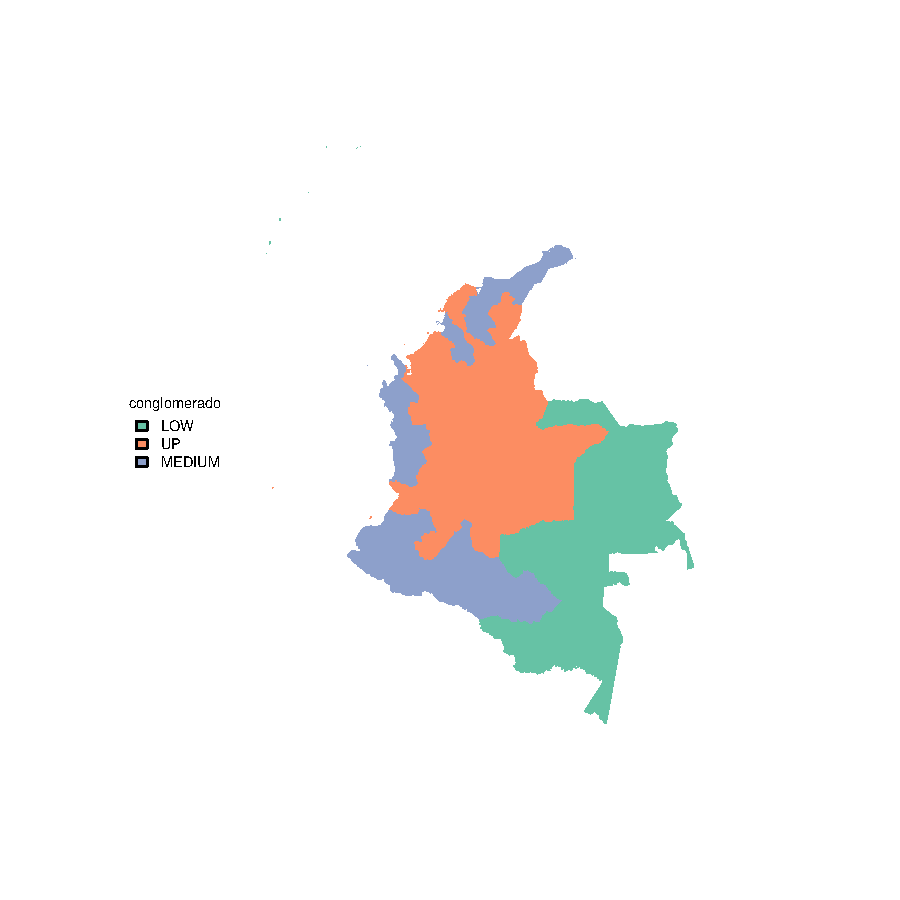
\includegraphics{ProyectoHC-plotMap1}
%\end{adjustbox}
\caption{Regiones conglomerados segun sus poblaciones}\label{clustmap}
\end{figure}
% 
\bibliographystyle{apalike}
\renewcommand{\refname}{Bibliografía}
\bibliography{Colombia}
%

\end{document}
